%%%%%%%%%%%%%%%%%%%%%%%%%%%%%%
%Documentclass Einstellungen %
%%%%%%%%%%%%%%%%%%%%%%%%%%%%%%

\documentclass[
    a4paper, %Papiergröße
    12pt, %Schriftgröße
    bibliography=totocnumbered, %Literaturverzereichnis als Eintrag ins Inhaltsverzeichnis
    twoside, %Zweiseitiger Druck
    %oneside, %Einseitiger Druck	
    BCOR=1cm, %Platz zum Lochen
]{scrartcl}


%%%%%%%%%%%%%%%%%%%%%%%%%%%%%%%%%%%%%%
% Geladene Dateien, für mehr ordnung %
%%%%%%%%%%%%%%%%%%%%%%%%%%%%%%%%%%%%%%
\usepackage{import/packages, import/commands, import/setup, import/details-titelseite}
\graphicspath{ {bilder/} }
\addbibresource{Literaturverzeichnis/literatur.bib}
% Zu beachten ist:
% >> packages sind alle im Protokoll benutzen Packete
% >> setup sind alle Einstellungen des Protokolls wie pagelayout, packeteinstellungen usw.
% >> commands sind eigen erstellte commands, um das lange tippen zu sparen
% >> details-titelseite hier befinden sich die Details, wie Versuchsdatum, Assistent, Teilnehmer, Versuchsnummer, usw. muss unbedingt ausgefüllt werden!





%%%%%%%%%%%%
% Dokument %
%%%%%%%%%%%%

\begin{document}
	
	
	%%%%%%%%%%%%%%
	% Titelseite %
	%%%%%%%%%%%%%%
	\thispagestyle{empty} % Auf Titelseite kein pagestyle, sodass man diese selbst gestalten kann
	
	\begin{titlepage}
		% Die ganzen Makros wie \VERSUCHSNAME, \VerfasserEINS, usw sind in der Datei details.sty auszufüllen!
		\begin{center}
			\Huge{\textbf{\VERSUCHSNR\ - \VERSUCHSNAME}}\\% \Huge \huge \Large \normalsize \Small usw. bestimmt die Schriftgröße.
			\vspace{10mm}% Abstand
			\Large{Protokoll zum Versuch des Physikalischen Praktikums I von \\ \textbf{\VerfasserEINS\;\& \VerfasserZWEI}}\\
			\vspace{10mm} 
			\Large{Universität Stuttgart}\\
		\end{center}
		\vspace{1cm}
		\begin{center}
			\begin{tabular}{ll}
				\large{Verfasser:}		& \large{\VerfasserEINS\;(\StudiengangEINS),} \\ 
				& \large{\MatNoEINS} \\
				\vspace{0cm}\\
				& \large{\VerfasserZWEI\;(\StudiengangZWEI),} \\
				& \large{\MatNoZWEI} \\
				\vspace{0cm}\\
				\large{Gruppennummer:}	& \large{\GRUPPENNR} \\
				\vspace{0cm}\\
				\large{Versuchsdatum:}	& \large{\VERSUCHSDATUM} \\
				\vspace{0cm}\\
				\large{Betreuer:}		& \large{\BETREUER}
			\end{tabular}
		\end{center}
		\vspace{15mm}
		
		\begin{center}
			Stuttgart, den \PROTOKOLLDATUM
		\end{center}
		
	\end{titlepage}
	
	
	%%%%%%%%%%%%%%%%%%%%%%%
	% Inhaltsverzeichniss %
	%%%%%%%%%%%%%%%%%%%%%%%
	
	\thispagestyle{empty}
	
	\tableofcontents 
	
	\clearpage %Neue Seite, davor werden alle noch ausstehenden Grafiken/Tabellen platziert.
	
	% Ab hier wollen wir nochmals neu die Seiten nummerieren, es fängt wieder mit Seite 1. an
	\renewcommand{\thepage}{\arabic{page}}
	\setcounter{page}{1}
	



    
	%%%%%%%%%%%%%%%%%%%%
	% Beginn Protokoll %
	%%%%%%%%%%%%%%%%%%%%
	
	
	%%%%%%%%%%%%%%%%%
	% Versuchsziele %
	%%%%%%%%%%%%%%%%%
	
	% Die erste eckige Klammer ist optional, die darin angegebene Bezeichnung steht im Inhaltsverzeichnis anstelle des hinteren (längeren) Namens.
	\section[Versuchsziel]{Versuchsziel und Versuchsmethode}
        
	
	%%%%%%%%%%%%%%
	% Grundlagen %
	%%%%%%%%%%%%%%
	
	\section[Grundlagen]{Grundlagen}
	   Das hier ist eine modifizierte Kopie der \LaTeX-Vorlage für Protokolle des Anfängerpraktikums der Universität Stuttgarts \cite{homepage}.
	
	%%%%%%%%%%%%%%%%%%
	% Messprinzipien %
	%%%%%%%%%%%%%%%%%%
	
	\section[Messprinzip]{Messprinzip mit Skizze und Versuchsablauf}
	
    	\subsection{Aufbau und Geräte}
            % Hier wird der Grobe aufbau aufgelistet, an besten mit Skizze
    	
    	\subsection{Versuch} 
	
	
	%%%%%%%%%%%%%
	% Messwerte %
	%%%%%%%%%%%%%
	
	\section[Messwerte]{Messwerte}

        \begin{table}[H]
            \centering
            \caption{
                Dies ist eine Beispieltabelle für die Messwert Sektion.
                Es empfiehlt sich alle Tabellen ungefähr im gleichem Stil zu bewahren.
                Der Tabellentyp S ist von \texttt{siunitx} und Formatiert die Nummern direkt richtig.
                Mit [table-number-alignment=left] hinter dem S, kann ausgesucht werden, wie die Nummern ausgerichtet werden.
                Zu sehen ist auch, dass die Nummer am Dezimaltrennzeichen ausgerichtet sind.
            }
            \begin{tabular}{c S}
                \toprule
                Beschreibung & {Messwert} \\
                A & 23.44 \\
                \midrule
                B & 463.25 \\
                \midrule
                C & 1712.53 \\
                \bottomrule
            \end{tabular}
            \label{tab:beispieltabelle}
        \end{table}

	
	%%%%%%%%%%%%%%
	% Auswertung %
	%%%%%%%%%%%%%%
	
	\section{Auswertung}
        Die Auswertung soll in mehrere Unterkapitel getrennt werden, je ein Kapitel pro Auswertungsziel.

        \subsection{Cooler Plot}
            In diesem Unterkapitel wird ein Plot erstellt.
            Ziel dieses Plots ist es die Funktion $1/\sqrt{x}$ zu untersuchen und deren Eigenschaften zu ermitteln.
            
            \begin{figure}[H]
                \centering
                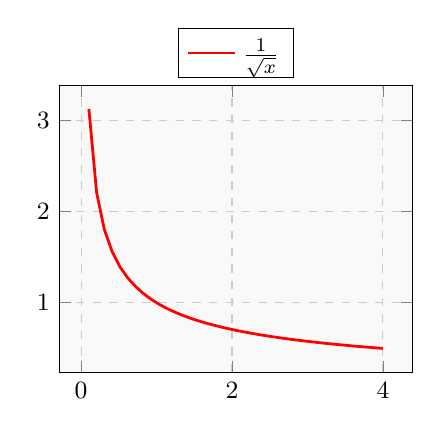
\begin{tikzpicture}%, trim axis right]
                    \begin{axis}[
                        width=0.5\linewidth, % Scale the plot to \linewidth
                        grid=major, % Display a grid
                        grid style={dashed,gray!40}, % Set the style
                        axis background/.style={fill=gray!5},
                        scaled y ticks=true,
                        tick label style = {font=\small},
                        every axis label/.style = {font=\small},
                        legend style={at={(0.5,1.2)},anchor=north,legend columns = 0}, % Legende über dem Plot
                    ]
                    
                    \addplot+ [
                        mark=none,
                        line width=1pt,  % Dünnere Linie
                        domain=0:4,    % x-Bereich
                        samples=40,       % Nur 2 Punkte für straight line (super dünn und effizient)
                        color=red
                    ] { 1/sqrt(x) };
                    \addlegendentry{$\frac{1}{\sqrt{x}}$} % Eintrag für die Legende
                \end{axis}
                \end{tikzpicture}
                \label{fig:beispielplot}
                \caption{
                    Plot der Funktion $f(x) = \frac{1}{\sqrt{x}}$.
                    Erstellt über das TikZ und pgfplot Paket.
                }
            \end{figure}

            Das ist ein \enquote{dummy}-Text, ihn durchlesen hat keinen Wert.
            Er dient nur zu Testzwecken.
            Hier auch als Test eine Inline Mathe $\frac{1}{2}$ okay!
            
	
	
	%%%%%%%%%%%%%%%%%%
	% Fehlerrechnung %
	%%%%%%%%%%%%%%%%%%

	\section[Fehlerrechnung]{Fehlerrechnung}
        \begin{equation}
            \Delta A = \ffp{A}{B} + \ffp{A}{C}
        \end{equation}

        \subsection{Fehlerdiskussion}

	
	%%%%%%%%%%%%%%%%%%%
	% Zusammenfassung %
	%%%%%%%%%%%%%%%%%%%
	
	\section[Zusammenfassung]{Zusammenfassung}
	
	
	\clearpage
	%%%%%%%%%%%%%%%%%%%%%%%%%%
	%%%Literaturverzeichnis%%%
	%%%%%%%%%%%%%%%%%%%%%%%%%%
	
	\printbibliography

	\clearpage
	%%%%%%%%%%
	% Anhang %
	%%%%%%%%%%
	
    \section{Anhang}
        % Hier kommt das Messwertblatt rein
        %\includepdf[pages=-]{Dateiname.pdf}
	
\end{document}